\chapter{Resultados}\label{cap:results}

\section{Experimentos}

\begin{figure}
    \centering
    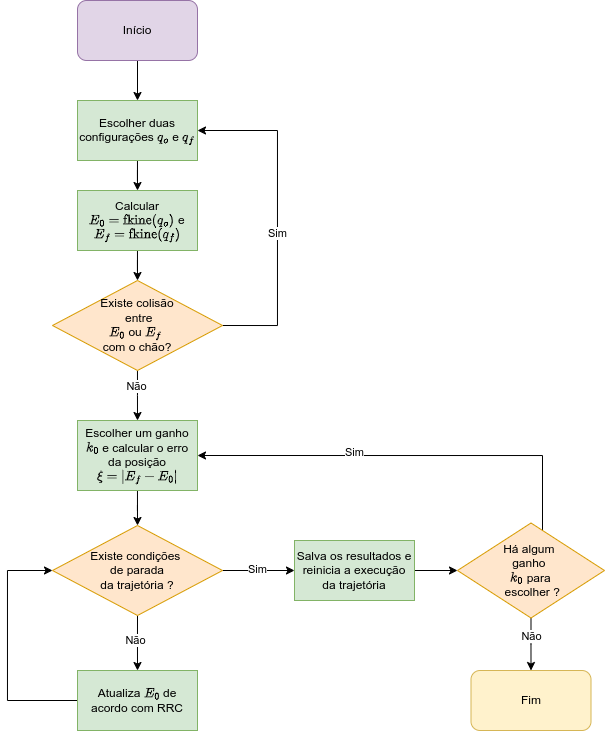
\includegraphics[width=0.8\textwidth]{./Images/exp-flow.png}
    \caption{Etapas seguidas na execução de um experimento.}\label{fig:exp-flow}
\end{figure}

\subsection*{Experimento 1}

$q_0 = q_f$ (variação de métrica controla o tempo de execução)

\subsection*{Experimento 2}

$q_0 \neq q_f$ (erro da posição e variação de métrica controla o tempo
de execução)

\subsection*{Experimento 3}
$q_0 = q_0 + q_0^\prime \neq q_f$ com $q_0^\prime \sim \mathcal{N}(0, 0.1)$ (erro da posição e variação de métrica
controla o tempo de execução) e repetir 100x

\begin{figure}
    \centering
    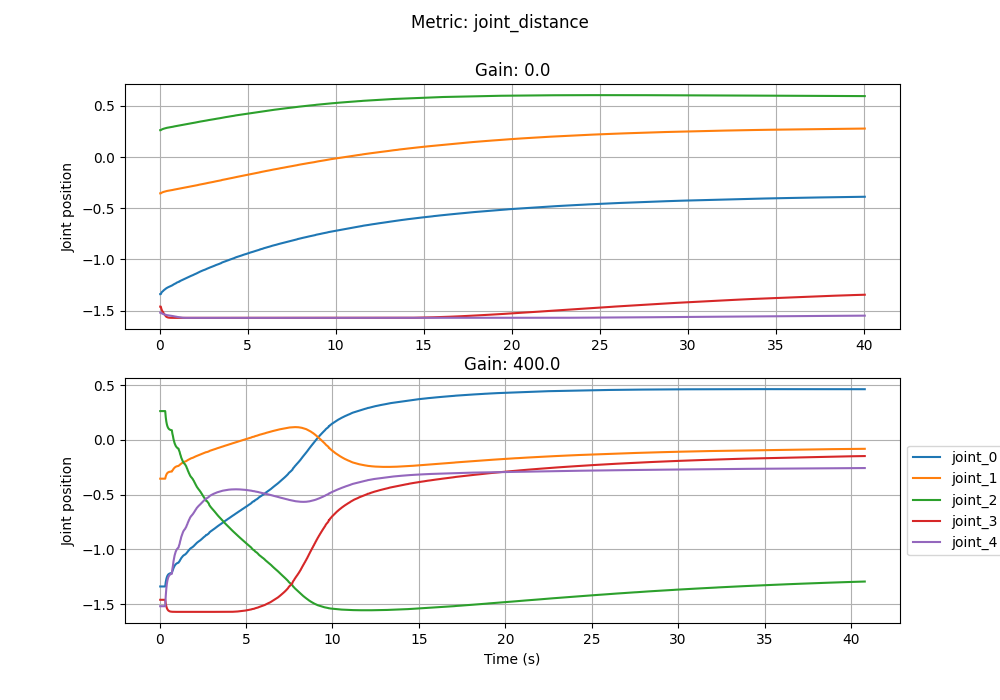
\includegraphics[width=1.0\textwidth]{Images/joint_distance/joint_states_joint_distance.png}
    \caption{Resultados}\label{fig:jd-js}
\end{figure}

\begin{figure}
    \centering
    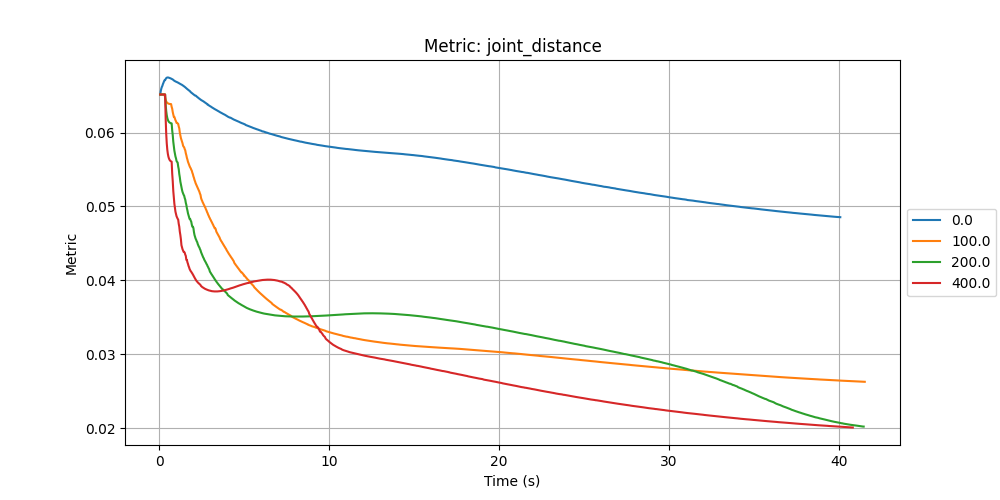
\includegraphics[width=1.0\textwidth]{Images/joint_distance/metric_joint_distance.png}
    \caption{Resultados}\label{fig:jd-m}
\end{figure}

\begin{figure}
    \centering
    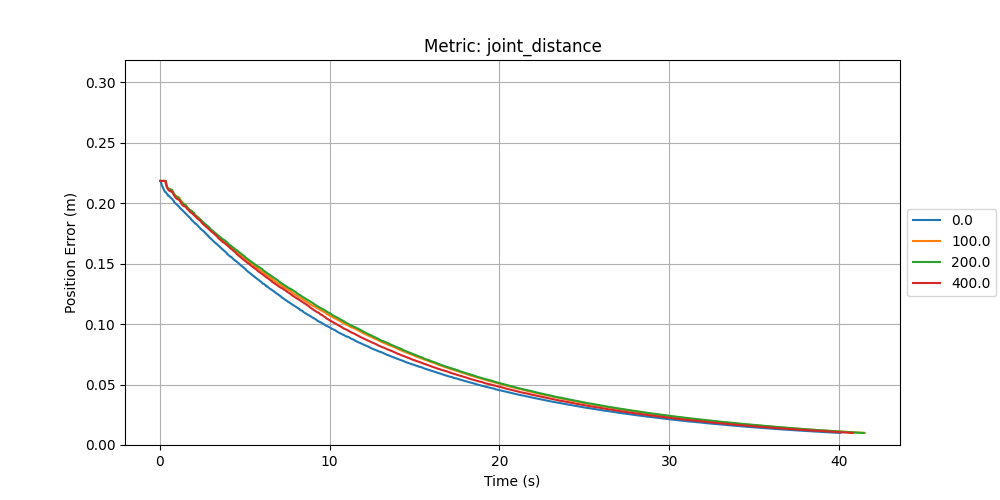
\includegraphics[width=1.0\textwidth]{Images/joint_distance/position_error_joint_distance.png}
    \caption{Resultados}\label{fig:jd-e}
\end{figure}

\begin{figure}
    \centering
    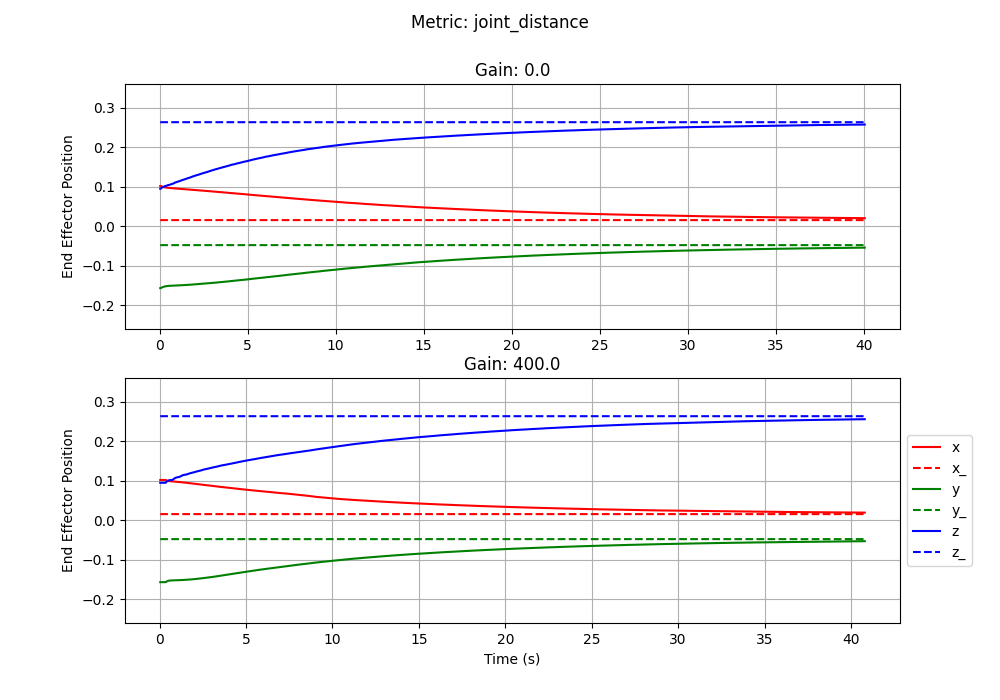
\includegraphics[width=1.0\textwidth]{Images/joint_distance/position_joint_distance.png}
    \caption{Resultados}\label{fig:jd-p}
\end{figure}

\begin{figure}
    \centering
    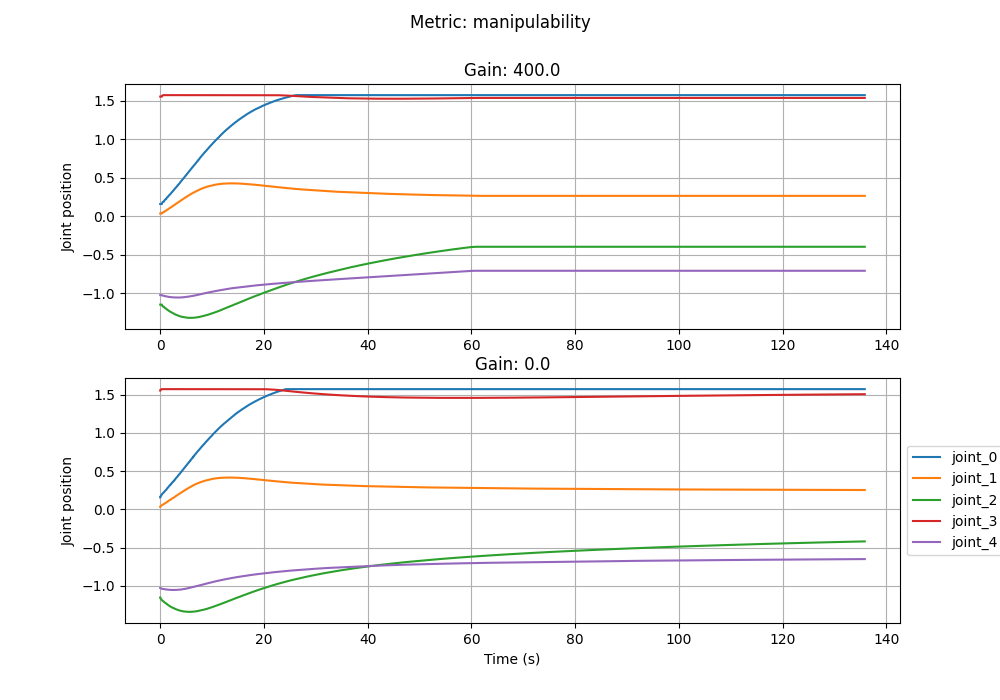
\includegraphics[width=1.0\textwidth]{Images/manipulability/joint_states_manipulability.png}
    \caption{Resultados}\label{fig:m-js}
\end{figure}

\begin{figure}
    \centering
    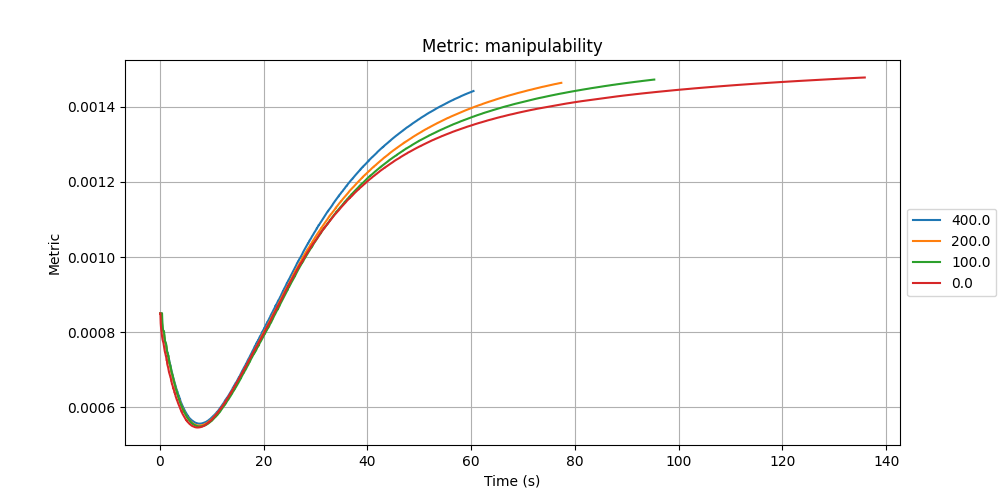
\includegraphics[width=1.0\textwidth]{Images/manipulability/metric_manipulability.png}
    \caption{Resultados}\label{fig:m-m}
\end{figure}

\begin{figure}
    \centering
    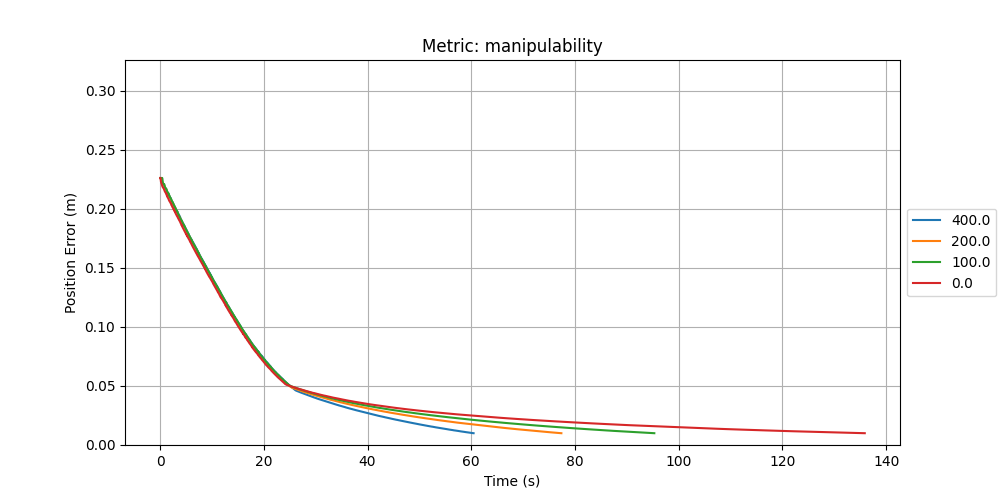
\includegraphics[width=1.0\textwidth]{Images/manipulability/position_error_manipulability.png}
    \caption{Resultados}\label{fig:m-e}
\end{figure}

\begin{figure}
    \centering
    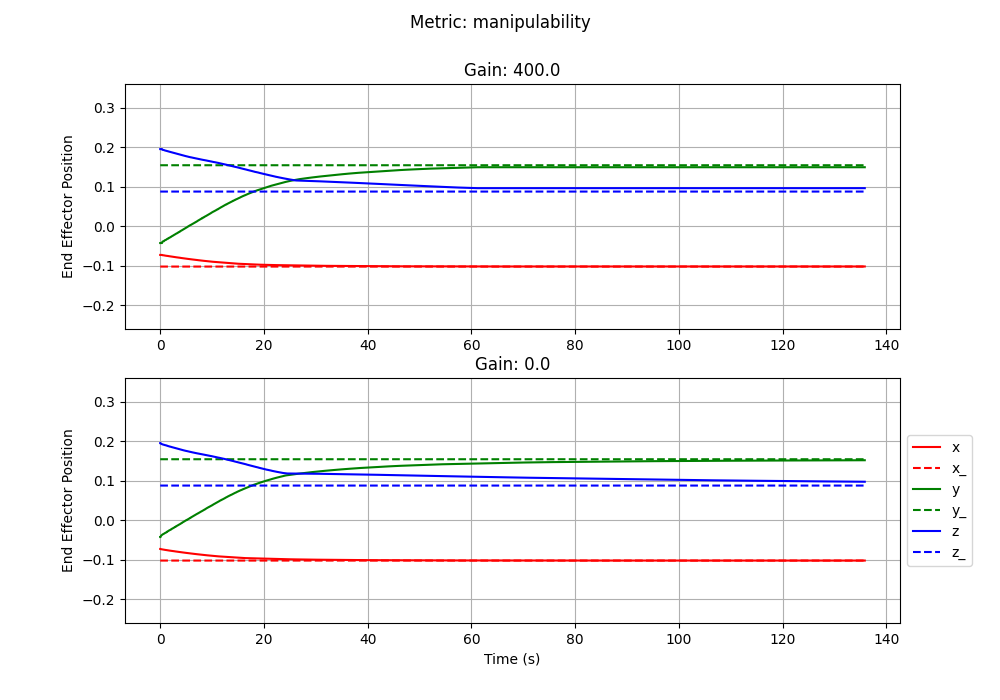
\includegraphics[width=1.0\textwidth]{Images/manipulability/position_manipulability.png}
    \caption{Resultados}\label{fig:m-p}
\end{figure}
